\documentclass[a4paper]{article}
\usepackage[spanish]{babel}
\usepackage[utf8]{inputenc}
\usepackage{amsmath}
\usepackage{listings}
\usepackage{xcolor}
\usepackage{amsfonts}
\usepackage{amssymb}
\usepackage[pdftex]{hyperref}
\usepackage{graphicx}

\begin{document}
    \title{\textbf{Proyecto \#1 DAA:} Procastinaci\'on ++}
    \author{L\'azaro Daniel Gonz\'alez Mart\'inez y Alejandra Monz\'on Pe\~na}
    \date{}
    \maketitle

    \section*{Desccripci\'on del problema}
    Sean las cadenas $S$, $T$ y una cadena vac\'ia $A$, se construyen nuevas cadenas de la siguiente forma: 

    \begin{itemize}
        \item[$\diamond $] Quitar la primera letra de $S$ y ponerla al inicio de la cadena $A$.
        \item[$\diamond $] Quitar la primera letra de $S$ y ponerla al final de la cadena $A$.    
    \end{itemize}

    Estas operaciones se pueden realizar hasta que $S$ quede sin caracteres.\\ 

    Se desea contar cuántas cadenas diferentes se pueden crear con estas operaciones tales que $T$ sea prefijo de 
    la nueva cadena ($A$).\\ 

    Definimos por comodidad la construcci\'on de cadenas combinando de cualquier forma posible las dos operaciones permitidas como 
    \textit{construcci\'on por aburrimiento}.

    \section*{Soluci\'on Backtrack}
    Una primera soluci\'on al problema planteado se puede obtener haciendo una exploraci\'on por todas las posibles cadenas que se pueden formar 
    y en cada caso comprobar si $T$ es prefijo de dicha cadena. 

    		% Configuración de Listings
	\lstset{keywordstyle=\color{blue}, basicstyle=\small}

	\begin{figure}[htb]
	
    \begin{lstlisting}[language=Python]

        def Procastinacion(S,T):
            if len(T) > len(S):
                return 0
            return Procastinacion2(S,T,'',0)
        
        def Procastinacion2(S,T,A,i):
            m = len(T)
            k = len(A)
            if len(S) <= i:
                return T == A[0:m]
            return Procastinacion2(S,T,f'{A}{S[i]}',i+1) 
                        + Procastinacion2(S,T,f'{S[i]}{A}',i+1) 
                            + ((m <= k) and (T == A[0:m]))
	\end{lstlisting}
	\caption{Código python del backtrack.}
	\end{figure}

    Este algoritmo de soluci\'on, aunque efectivo es demasiado costoso computacionalmente, sean $|S| = n$ y $|T| = m$, se tiene que:

    \begin{equation*}
        T(n,m) = 2 T(n-1) + m 
    \end{equation*}

    de donde, al utilizar el Teorema Maestro para funciones decrecientes, se obtiene para este problema que 
     $T(n,m) = \Theta(2^n + m)$.

    \section*{Explotando caracter\'isticas del problema}
    Una primera mejora que se puede hacer, se basa en la idea de que la primera letra de $S$ 
    al poder colocarse tanto al inicio como al final de la cadena vac\'ia $A$, genera dos \'arboles de cadenas exactamente iguales (con las mismas cadenas), solo que estas se pueden considerar ``diferentes'' por 
    haber tenido un movimiento inicial distinto.\\ 

    Por tanto una mejora inicial, consiste en no duplicar innecesariamente el espacio de b\'usqueda, sino asumir que en $A$ inicialmente 
    est\'a el primer caracter de $S$ y duplicar el resultado final. Aunque esta idea no mejora la complejidad temporal, reduce a la mitad la cantidad de operaciones a realizar.

    \section*{Soluci\'on con Programaci\'on Din\'amica}

    Representando las cadenas $S$ y $T$ por sus caracteres, tenemos:

    \begin{itemize}
        \item[] $T$ = $T_0T_1 ... T_{m-1}$
        \item[] $S$ = $S_0S_1 ... T_{n-1}$ 
    \end{itemize}

    Entonces $T_i$ ($S_i$) denota al i-\'esimo m\'as un cararacter de $T$($S$), de igual modo 
    $T_{i...j}$($S_{i...j}$) denota a la subcadena $T_iT_{i+1}...T_j$ ($S_iS_{i+1}...S_{j}$) de la cadena $T$ ($S$).\\
    
    Definamos la funci\'on $f(i,j)$ como la cantidad de cadenas $A_{i...j}$ \textit{construidas por aburrimiento} con los primeros $j-i+1$ 
    caracteres de S (es decir con los caracteres de $S_{0...j-i}$) donde 
    para:
    \begin{itemize}
    	\item[i] $j < m$, $\quad A_{i...j} = T_{i...j}$
    	\item[ii] $j \geq m $ y $i < m $, $\quad A_{i...j} = T_{i...m-1}A_{m...j}$
    	\item[iii] $i > m $, $\quad A_{i...j} = A_{i...j}$
    \end{itemize}
    
    Luego $\sum_{j= m-1}^{n-1}f(0,j)$ es la cantidad total de cadenas que se pueden \textit{construir por aburrimiento} que tienen como prefijo a $T$.\\
    
    Notemos qu\'e, para $i < m$ se cumple que: %TODO:

    \begin{equation}\label{eq:1}
        f(i,i) = \left\{ \begin{aligned}
            &2, &T_i = S_0\\
            &0, &eoc
        \end{aligned} \right.
    \end{equation}

    Esto se debe a que, como queremos formar subcadenas de tama\~no 1 de $T$ con el primer caracter de $S$, tenemos en los casos que hay coincidencia (\ref{fig:ppp1}), dos maneras de colocar el caracter, (por delante y por detr\'as) y en los restantes casos 
    se tiene 0 puesto que no se tiene ninguna subcadena de $T$ de longitud 1 al tomar ese caracter (\ref{fig:ppp0}).\\
        
    \begin{figure}[!h]
    	\label{fig:ppp1}
    	\centering
    	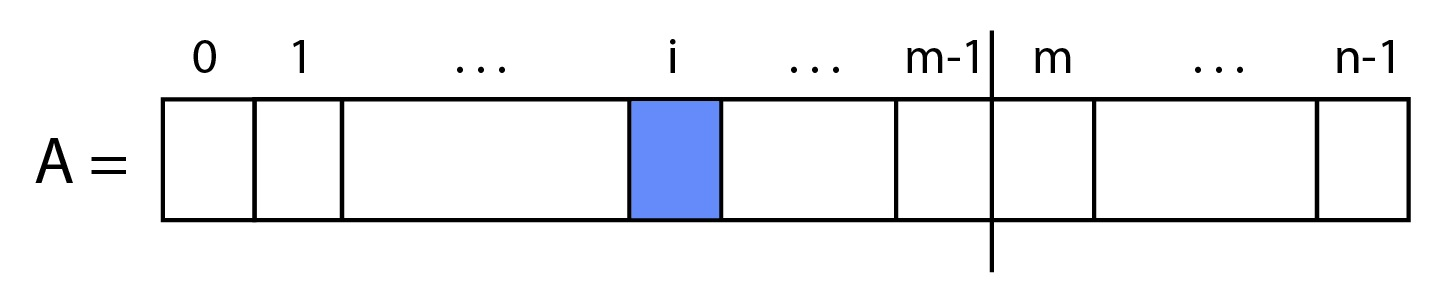
\includegraphics[width=0.7\linewidth]{ppp1}
    	\caption{}
    \end{figure}

	\begin{figure}[!h]
		\label{fig:ppp0}
		\centering
		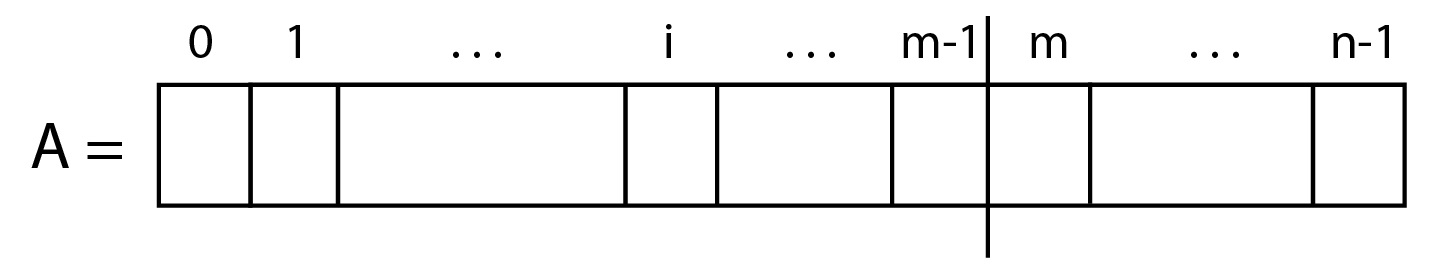
\includegraphics[width=0.7\linewidth]{ppp0}
		\caption{}
	\end{figure}

    
    
    Adem\'as se cumple, para $i \geq m$, que $f(i,i) = 2$, puesto que poner cualquier caracter en posiciones de $A$ mayores que el prefijo $T$ (\ref{fig:ppp2}) origina una cadena de longitud 1 válida para la definición de la función $f$ (iii) y el valor es 2, puesto que de igual modo este caracter se pudo colocar por delante o por atrás de la cadena vacía.\\
    
    \begin{figure}[!h]
    	\label{fig:ppp2}
    	\centering
    	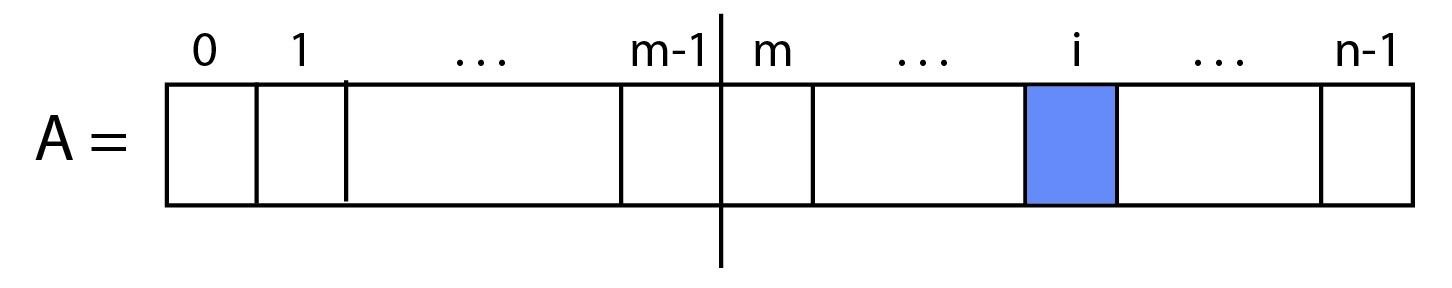
\includegraphics[width=0.7\linewidth]{ppp2}
    	\caption{}
    \end{figure}
     

    A modo general $f(i,j)$ se puede construir recursivamente como: 

    \begin{equation*}
        f(i,j) = f(i+1,j)\mathbb{I}_{ \{T_i = S_{j-i+1} \vee i \geq m \}}  +  f(i,j-1)\mathbb{I}_{ \{T_j = S_{j-i+1} \vee j \geq m \} } 
    \end{equation*}

    Ya que $S_{j-i+1}$ se puede agregar por delante a las cadenas $A_{i+1}...A_j$ (\ref{fig:ppp3}), o por atr\'as a las cadenas 
    $A_{i}...A_{j-1}$ (\ref{fig:ppp4}), cuando $S_{j-i+1}$ coincide con $T_i$ o $T_j$ respectivamente, formando as\'i cadenas $A_{i}...A_{j}$.\\
    
    \begin{figure}[h!]
    	\label{fig:ppp3}
    	\centering
    	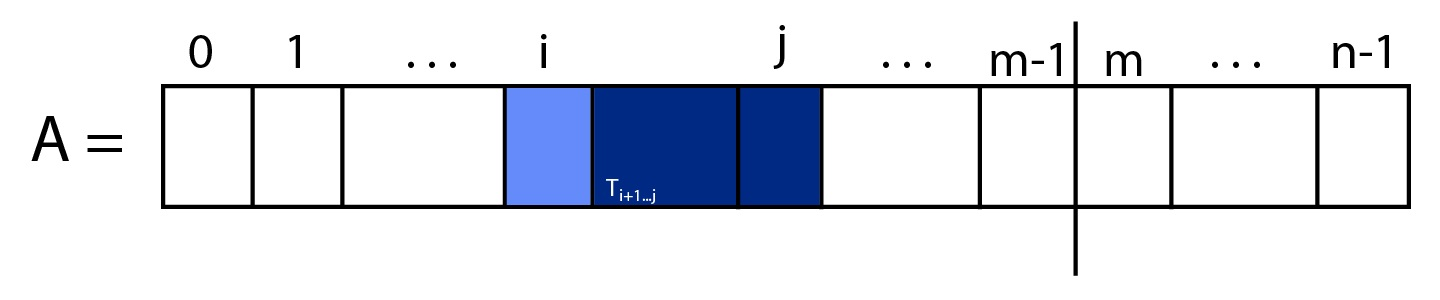
\includegraphics[width=0.7\linewidth]{ppp3}
    	\caption{}
    \end{figure}
    \begin{figure}[h!]
        \label{fig:ppp4}
    	\centering
    	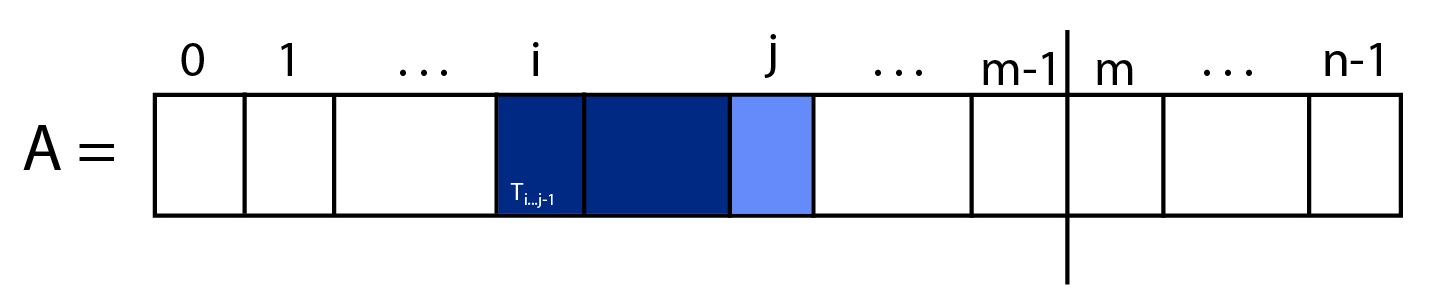
\includegraphics[width=0.7\linewidth]{ppp4}
    	\caption{}
    \end{figure}
    

    En los casos (ii), a la subcadena $A_{i...j-1}$ se le puede agregar el caracter $S_{j-i+1}$ por atr\'as sin afectar 
    el prefijo (\ref{fig:ppp5a}), generando la cantidad de cadenas que hab\'ia en $f(i,j-1)$, pero ahora de la forma $A_{i...j}$. Note que esta condición no implica que no se pueda cumplir que $T_{i} =  S_{j-i+1}$ por lo que en este caso podría ponerse por delante sin problema (\ref{fig:ppp5}).\\
    
    \begin{figure}[h!]
    	\centering
    	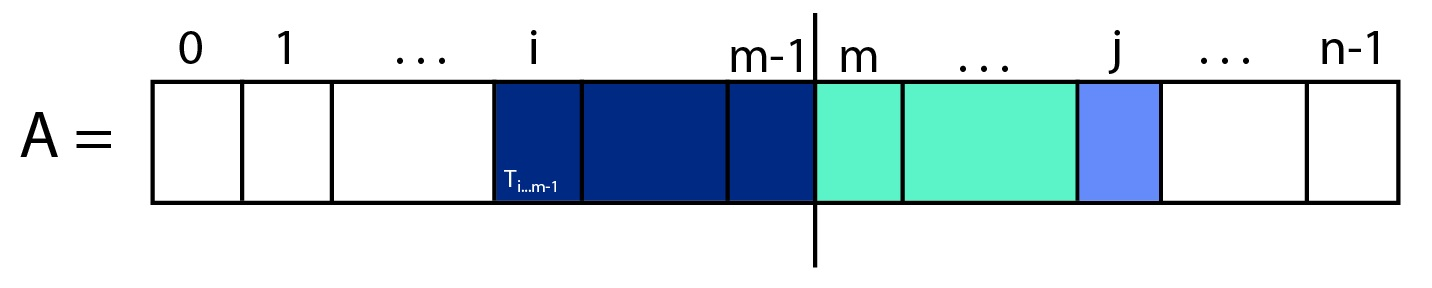
\includegraphics[width=0.7\linewidth]{ppp5a}
    	\caption{}
    	\label{fig:ppp5a}
    \end{figure}

	\begin{figure}[h!]
		\centering
		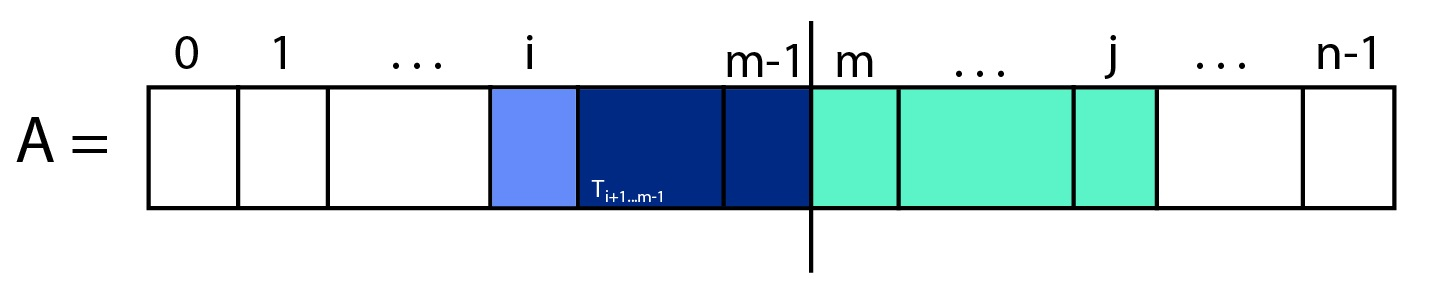
\includegraphics[width=0.7\linewidth]{ppp5}
		\caption{}
		\label{fig:ppp5}
	\end{figure}
    
    
    Por \'ultimo cuando $i \geq m$ entonces $j \geq m$ y se puede agregar $S_{j-i+1}$ como prefijo de 
    $A_{i+1...j}$ (\ref{fig:ppp6}) y como sufijo de $A_{i...j-1}$ (\ref{fig:ppp7}) cayendo en el caso (iii), por lo tanto tendr\'iamos $f(i+1,j) + f(i,j-1)$ cadenas de la forma $A_{i...j}$.
    
    \begin{figure}[h!]
    	\centering
    	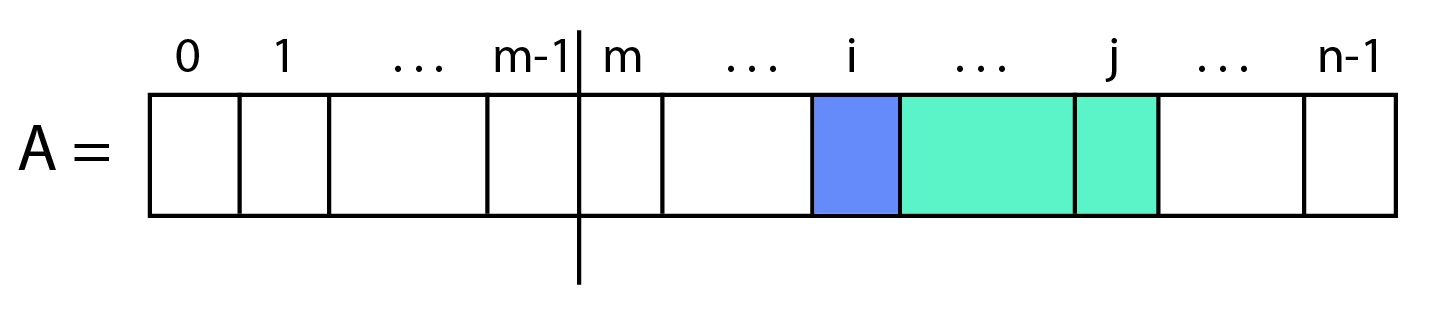
\includegraphics[width=0.7\linewidth]{ppp6}
    	\caption{}
    	\label{fig:ppp6}
    \end{figure}
    \begin{figure}[h!]
    	\centering
    	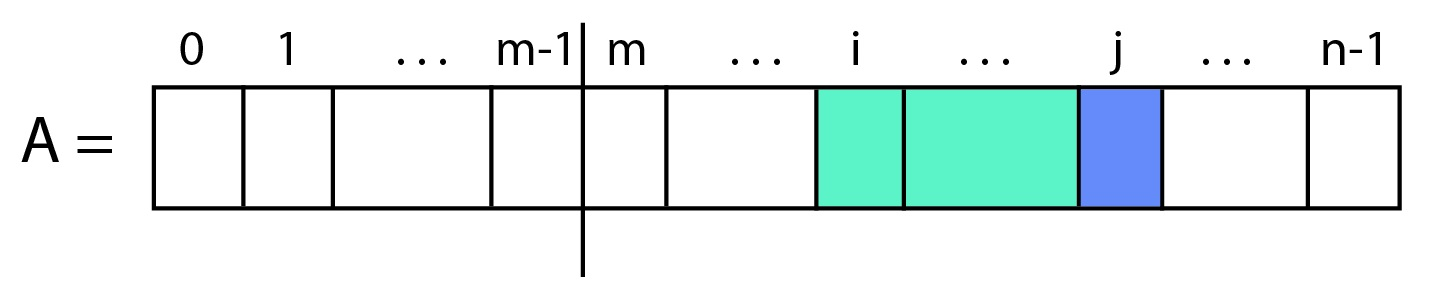
\includegraphics[width=0.7\linewidth]{ppp7}
    	\caption{}
    	\label{fig:ppp7}
    \end{figure}

\section*{Implementación de la dinámica}
    
    
    \begin{lstlisting}[language=Python]
def solve_dp(S,T):
    n = len(S)
    m = len(T)
        
    if m > n:
        return 0
        
    dp = [[0 for j in range(n)] for i in range(n)]
    
    for i in range(n):
        if i >= m or T[i] == S[0]:
            dp[i][i] = 2
    
    for k in range(1, n):    
        c = S[k]
        
        i = 0        
        for j in range(k, n):
            if i >= m or c == T[i]:
                dp[i][j] += dp[i+1][j]
            if j >= m or c == T[j]:
                dp[i][j] += dp[i][j-1]            
            i += 1            
    
    return sum(dp[0][m-1:])
    \end{lstlisting}
	
	\section*{Correctitud del algoritmo}
	
	Como nos queda claro que $\sum_{j= m-1}^{n-1}f(0,j)$ es la respuesta a nuestro problema, demostrar que $dp[i][j] = f(i,j)$, sería suficiente para probar la correctitud del algoritmo. Por lo tanto demostremos que en el momento que se actualiza el valor de $dp[i][j]$ este coincidirá con $f(i,j)$.
	
	Hagamos inducción en la longitud de la cadena que estamos formando $A_{i...j}$, lo que es equivalente a hacer la inducción sobre el ciclo en que itera $k$.
	
	\begin{itemize}
		\item Caso base: $|A_{i...j}| = 1$
		
		Como por definición, $i \leq j$ entonces $|A_{i...j}| = 1$ si y solo si $i = j$, ya que $|A_{i...j}| = j-i + 1 = 1$.
		Luego todas las cadenas que puedan pertenecer a nuestro caso base están en la diagonal de $dp$, y se inicializan atendiendo a la definición de $f(i, i)$ dada en (\ref{eq:1}), entonces tenemos que:
		$$dp[i][i] = f(i, i)$$.
		Note que se inicializan así en el ciclo que itera por $i$ del código.
		
		\item Caso Hipótesis: Supongamos que para toda cadena $A_{i^\prime...j^\prime}$ de tamaño menor que $p$ se cumple que $dp[i^\prime][j^\prime] = f(i^\prime, j^\prime)$ con $j^\prime - i^\prime + 1 < p$. Esto es equivalente a que hasta la iteración $p-1$ del ciclo que itera sobre $k$, se cumple que lo planteado anteriormente\footnote{Observe que, para que la fórmula tenga sentido, $i^\prime \leq j^\prime$}.
		
		Sea $A_{i...j}$ de tamaño $p$. Podemos asumir $i<j$, porque el caso base ya está tratado a parte. Luego como
		$$f(i,j) = f(i+1,j)\mathbb{I}_{ \{T_i = S_{j-i+1} \vee i \geq m \}}  +  f(i,j-1)\mathbb{I}_{ \{T_j = S_{j-i+1} \vee j \geq m \} } $$
		se aprecia que $f(i,j)$ depende de los valores de $f(i+1,j)$ y $f(i,j-1)$. Luego como $|A_{i+1...j}| = j-(i+1) + 1 = j-i$, y $j-i < p$, entonces por hipótesis $f(i+1,j) = dp[i+1][j]$. De manera similar como $|A_{i...j-1}| = j-1 - i + 1 = j-i < p$, aplicamos la hipótesis pero en este caso $f(i,j-1) = dp[i][j-1]$.
		Luego
		$$f(i,j) = dp[i+1][j]\mathbb{I}_{ \{T_i = S_{j-i+1} \vee i \geq m \}}  +  dp[i][j-1]\mathbb{I}_{ \{T_j = S_{j-i+1} \vee j \geq m \} } $$
		y finalmente $dp[i][j]$ al actualizarse con este cálculo nos quedará:
		$$dp[i][j] = f(i,j)$$				
	\end{itemize}

	Luego por Principio de Inducción Matemática demostramos que al concluir el algoritmo queda computado para cada $dp[i][j]$, con $0 \leq i\leq j < n$, la cantidad de cadenas $A_{i...j}$ que se pueden \textit{construir por aburrimiento} con los primeros $|A_{i...j}| = j-i+1$ caracteres de $S$, es decir, queda guardado en $dp[i][j]$ el valor de $f(i,j)$.	
	



	\section*{Complejidad Temporal}
	
	Definir e inicializar la matriz $dp$ se hace en $2n^2$ operaciones ya que esta tiene dimensión $n \times n$.
	
	El ciclo que itera por $k$ ejecuta el ciclo que itera por $j$, unas $n-1$ veces. Y este ciclo se ejecuta $n-k$ veces para la iteración $k$. Es decir, ambos ciclos ejecutan un total de veces igual a:
	$$ \sum_{k=1}^{n-1} (n-k) = (n-1) + (n-2) + ... + 1 = \frac{n(n-1)}{2} $$
	
	Finalmente cuando se calcula la suma de los $dp[0][i]$ para $i \geq m$, se hacen $n-m + 1$ iteraciones.
	
	Por lo tanto al sumar cada uno de estos costos considerando también, el tiempo constante que requieren las operaciones intermedias, nos quedaría algo así:
	
	$$T(n,m) = c_1 + 2n^2 + c_2\frac{n(n-1)}{2} + n-m+1$$
	
	Demostremos que $T(n,m)$ es $O(n^2)$:
	
	Para esto debemos encontrar una constante $C$ tal que a partir de cierto $n$, se cumpla $T(n,m) \leq Cn^2$.
	$$T(n,m) \leq c_1 + 2n^2 + c_2\frac{n(n-1)}{2} + n + 1$$
	
	Calculemos el límite:
	$$ \lim_{n}\left(\frac{c_1 + 2n^2 + c_2\frac{n(n-1)}{2} + n + 1}{n^2}\right)$$
	$$= \lim_{n}\left(\frac{2c_1 + 4n^2 + c_2n(n-1) + 2n + 2}{2n^2}\right)$$
	$$= \frac{4+c_2}{2}$$
	Como este límite es finito y mayor que $0$, existirá una constante $C$ tal que :
	$$ c_1 + 2n^2 + c_2\frac{n(n-1)}{2} + n + 1 \leq Cn^2$$
	y por transitividad, $ T(n,m) \leq Cn^2 $. Luego $T(n,m)$ es $O(n^2)$.
	
	Incluso si queremos ser más exquisitos podemos demostrar que $T(n,m) = \theta(n^2)$. \\
	
	Como:
	$$c_1 + 2n^2 + c_2\frac{n(n-1)}{2} \leq T(n,m)$$
	Calculando el límite siguiente:
	$$ \lim_{n}\left(\frac{c_1 + 2n^2 + c_2\frac{n(n-1)}{2}}{n^2}\right)$$
	$$= \lim_{n}\left(\frac{2c_1 + 4n^2 + c_2n(n-1)}{2n^2}\right)$$
	$$= \frac{4+c_2}{2}$$
	De forma similar, existirá una constante $C$ tal que a partir de cierto $n$, se cumple que 
	$$Cn^2 \leq c_1 + 2n^2 + c_2\frac{n(n-1)}{2}$$
	y por transitividad se cumple que $Cn^2 \leq T(n,m)$. Luego $T(n,m) = \Omega(n^2)$. Y finalmente $T(n,m)$ es $\theta(n^2)$.
	
    \section*{Y si te dijera que esto se puede mejorar??}
    Al analizar numerosos casos, pudimos comprobar que en muchos de ellos, el primer caracter de $S$, $S_0$ no estaba presente en la cadena $T$, por tanto 
    luego de poner este caracter en $A$ hab\'ia solo una de las dos opraciones posibles para formar el prefijo $T$ en $A$ y es poner todo caracter de 
    $T$ en $A$ con movimientos hacia alante.\\ 

    (Dem) Sea una cadena $A$, con prefijo $T$,creada a partir de una cadena $S$, cuyo primer caracter $S_0$ no pertenezca al alfabeto de $T$, 
    supongamos que en el prefijo $T$ de $A$, alg\'un caracter se coloc\'o con un movimiento hacia atr\'as. Sea 
    $S_k$ ese caracter, entonces como se puso con un movimiento hacia atr\'as, la posici\'on $j$ de $S_k$ en $A$
    es mayor que la posici\'on de $S_0$ en $A$. Como asumimos que $S_k$ est\'a en el prefijo $T$ de $A$, entonces todo otro caracter anterior 
    a $S_k$ en $A$ tiene que estar en el prefijo $T$, por lo tanto $S_0$ tendr\'ia que estar en el prefijo, lo cual es una contradicci\'on. As\'i queda demostrado que 
    si $S_0$ no pertenece a las letras que forman a $T$, todas las cadenas $A$ que tengan a $T$ como prefijo construidas por aburimiento, 
    contruyen al prefijo solo con movimientos hacia adelante.\\

    De la demostraci\'on anterior se deduce que como solo se usan movimientos hacia alante, reverso del prefijo $T$ ha de ser subsecuencia de $S$.\\

    De esta observaci\'on percibimos que era posible obtener una soluci\'on al problema separando los modos de construcci\'on de prefijos 
    en una partici\'on: 

    \begin{itemize}
        \item Con cadenas cuyo prefijo $T$ se contruy\'o solo con movimientos hacia alante.
        \item Con cadenas cuyo prefijo $T$ se contruy\'o con al menos un movimiento hacia atr\'as.
    \end{itemize}

    \subsection*{Prefijo $T$ solo con movimientos hacia alante}

    Definamos la funci\'on $prefix(i,j)$ como la cantidad de prefijos de $T$ de longitud $j + 1$ que se pueden formar utilizando los \'ultimos $n - i$ caracteres de $S$ con movimientos hacia alante.\\ 

    Si hacemos un primer an\'alisis, nos podemos dar cuenta que:
    $$prefix(i,0) = \left\{ \begin{aligned}
        &0,& i = n \\
        & prefix(i+1,0) + n -i,& i < n~ y~ T_0=S_{n-i-1} \\
        &prefix(i+1,0), & eoc
    \end{aligned}\right.$$

    En el caso $i = n$ la cantidad de prefijos de longitud $1$ que se pueden hacer con $0$ caracters es evidentemente $0$.\\
    
    En el caso $i < n$ y $T_0=S_{n-i-1}$, como el caracter $S_{n-i-1}$ puede construir una cadena de longitud $1$ que sea prefijo de $T$ al ser agregado con un movimiento hacia alante a la cadena en formaci\'on; y 
    los $n-i-1$ caracteres finales de $S$ se pueden (o no) insertar hacia atr\'as (uno a uno) en la cadena en formaci\'on, se tendr\'ian $1 + (n-i-1) = n-i$ nuevas cadenas con prefijo de longitud $1$ de $T$.
    Adem\'as
    se tienen las formas que ya exist\'ian de construir cadenas con $n-(i+1)$ caracteres, es decir $prefix(i+1, 0)$.\\ 

    En el tercer caso, al no haber coincidencia de $S_{n-i-1}$ con $T_0$, la inclusi\'on de $S_{n-i-1}$ al ponerlo por delante, no genera nuevas cadenas con prefijos de longitud $1$ de $T$.
    Note que no tiene sentido poner estos caracteres por detr\'as hasta que no se tenga la seguridad
    de que exista un caracter que pueda formar el prefijo de longitud 1 de $T$, y si este caracter existe,
    en alguna posici\'on $k < n-i-1$ de $S$,
    m\'as adelante estos caracteres se incluir\'ian en $prefix(k, 0)$.
    Por tanto, hasta este punto se 
    mantiene que la cantidad de prefijos formados es la misma a la que se ten\'ia sin contar con $S_{n-i-1}$, es decir $prefix(i+1,0)$.\\
    
    Esto se puede representar como:
    $$
    \begin{aligned}
        &prefix(n,0) = 0\\
        &prefix(i,0) = prefix(i+1,0) + (n-i)\mathbb{I}_{\{ T_0 = S_{n-i-1}\}}
    \end{aligned}
    $$

    Luego con un an\'alisis similar se tiene que para $j > 0$:

    $$prefix(i,j) = \left\{ \begin{aligned}
        &0,& i = n \\
        & prefix(i+1,j) + prefix(i+1,j-1),& i < n~ y~ T_0=S_{n-i-1} \\
        &prefix(i+1,j), & eoc
    \end{aligned}\right.$$ 

    Trivialmente cuando $i=n$, la cantidad de prefijos de longitud $j+1$
    que se pueden hacer con los \'ultimos $0$ caracteres de $S$ es $0$.

    Cuando $i < n$ y $T_i = S_{n-i-1}$, se puede colocar por delante $S_{n-i-1}$ faltar\'ia poner las letras correspondientes
    al prefijo de $T$ de longitud $j$ para obtener el prefijo $T$ de longitud $j+1$, como en la cadena en formaci\'on hasta el momento se tienen que 
    haber puesto con los movimientos permitidos todos los caracteres de $S_{0... n-i-1}$, el prefijo de longitud $j$ que falta se debe pode hacer con los 
    restantes $n-i$ caracteres finales, es decir que se pueden obtener tantos como $prefix(i+1, j-1)$. Adem\'as se conservan las formas de hacer el prefijo de longitud $j+1$
    sin utilizar el caracter $S_{n-i-1}$ como parte del prefijo, o sea $prefix(i+1,j)$.\\

    En otro caso, solo se puede construir $T$ con lo que ya exist\'ia de la formaci\'on, es decir,
    sin utilizar $S_{n-i-1}$, se conservan las formas de hacer el prefijo de longitud $j+1$ ($prefix(i+1,j)$).

    \subsubsection*{Correctitud de la funci\'on \texttt{compute\_prefix}}

    Para obtener una representaci\'on computacional de la funci\'on $prefix$,
rellenamos una matriz $dp$ de $(n+1) \times m$ tal que $dp[i][j] = prefix(i,j)$. Utilicemos Inducci\'on Matem\'atica 
para demostrar la correctitud del algoritmo. Primero demostremos que $dp[i][0] = prefix(i,0)~\forall~n\leq i \leq 0$. \\


\begin{itemize}
    \item Caso Base: $i = n$
    Cuando $i=n$, $dp[n][0] = 0$ ya que la inicializaci\'on de la matr\'iz rellena $dp$ con $0$ por defecto (esto se cumple adem\'as para toda $j$). 
    y  $prefix(n,0)=0$ (en general $prefix(n,j) = 0$), de done $prefix(n,0)= dp[n][0]$.

    \item Caso Hip\'otesis: Supongamos que para $i = k$ se cumple que $dp[k][0] = prefix(k,0)$.\\ 
    
    Sea $i = k-1$, se tiene que $$prefix(k-1,0) = prefix(k,0) + (n-k+1)\mathbb{I}_{\{ T_0 = S_{n-k}\}}$$.
    Luego como $dp[k][0] = prefix(k,0)$ por hip\'otesis, entonces 
    $$prefix(k-1,0) = dp[k][0] + (n-k+1)\mathbb{I}_{\{ T_0 = S_{n-k}\}}$$ y precisamente la expresi\'on 
    $dp[k][0] + (n-k+1)\mathbb{I}_{\{ T_0 = S_{n-k}\}} $ es lo que se le asigna a $dp[k-1][0]$ en el c\'odigo, en el ciclo que 
    inicializa la matriz $dp$. Por tanto se tiene que $dp[k-1][0] = prefix(k-1,0)$.

\end{itemize}

Ya demostrado el caso para $j=0$ procedamos a demostrar con otra inducci\'on que $dp[i][j]$ es consistente con los valores de la funci\'on $prefix(i,j)$ para 
todos los restantes valores de $0 \leq j \leq i \leq n$

\begin{itemize}
    \item Caso Base: $j = 0$ 
    
    Como se demostr\'o en la inducción anterior para todo $n \leq i \leq 0$ se cumple que $dp[i][0] = prefix(i,0)$. 

    \item Caso Hip\'otesis: Supongamos que para $j = k$, para todos los valores $n \leq i \leq 0$, se cumple que $dp[i][k] = prefix(i,k)$.
    
    Sea $j = k+1$, sabemos que: $$prefix(i,k+1) = prefix(i+1,k+1) + prefix(i+1,k)\mathbb{I}_{\{ T_{k+1} = S_{n-i-1}\}}$$. Por hip\'otesis 
    sabemos que $prefix(i+1,k) = dp[i+1][k]$, faltar\'ia demostrar que $prefix(i+1,k+1) = dp[i+1][k+1]$. Hagamos una inducci\'on sobre $i$, manteniendo la columna actual 
    para demostrarlo. 

    \begin{itemize}
        \item Caso Base: $j = k+1$, $i = n$
        
        Como planteamos con anterioridad la inicializaci\'on de la matr\'iz rellena $dp$ con $0$ por defecto, por tanto  
        y  $prefix(n,k+1)=dp[n][k+1] = 0$. 

        \item Caso Hip\'otesis: Supongamos que $prefix(l,k+1) = dp[l][k+1]$. 
        
        Sea $i = l-1$, como $$prefix(l-1,k+1) = prefix(l,k+1) + prefix(l,k)\mathbb{I}_{\{ T_{k+1} = S_{n-l}\}}$$
        Por la hip\'otesis interna tenemos que $prefix(l,k) = dp[l][k]$,
        y por la hip\'otesis externa tenemos que $dp[l][k+1] = prefix(l,k+1)$

        Luego $$prefix(l-1,k+1) = dp[l][k+1] + dp[l][k]\mathbb{I}_{\{ T_{k+1} = S_{n-l}\}}$$
        y como $dp[l-1][k+1]$ se computa de esta forma, tenemos que:

        $$dp[l-1][k+1] = prefix(l-1,k+1)$$
    \end{itemize}

    Luego por Principio de Inducción Matemática queda demostrado que $prefix(i+1,k+1) = dp[i+1][k+1]$.
    De esta manera ahora se tiene que
    $$prefix(i,k+1) = dp[i+1][k+1] + dp[i+1][k]\mathbb{I}_{\{ T_{k+1} = S_{n-i-1}\}}$$
    Y finalmente como $dp[i][k+1]$ se calcula con este valor, entonces concluimos que
    $$prefix(i,k+1) = dp[i][k+1]$$
\end{itemize}
    Luego por Principio de Inducción Matem\'atica queda demostrado que $dp[i][j] = prefix(i,j)$.
    
    Entonces la cantidad de cadenas que se pueden formar con prefijo $T$ construido solo con
    movimientos hacia alante, con los caracteres de $S$ ser\'ia:

    $$ 2 \cdot \sum_{\forall i, T_{m-1} = S_i} (prefix(i,m-1) - prefix(i+1,m-1)) \cdot 2^{\max(i-1,0)} $$

    Note que $prefix(i,m-1) - prefix(i+1,m-1)$ representa del total de cadenas posibles,
    con prefijo $T$ construido solo con movimientos hacia adelante, aquellas que tienen como
    \'ultimo caracter de $T$ el caracter $S_i$. Observe que antes de $S_{i}$ podemos formar
    de cualquier forma (por aburrimiento) cadenas antes de empezar a formar el prefijo.
    La cantidad de formas para construir cadenas con los primeros $i-1$ caracteres ser\'ia
    colocar una a una las letras de $2$ formas: por delante o por detr\'as. Esto nos dar\'ia
    un \'arbol binario de profundidad $i-1$, en el cual la cantidad de cadenas ser\'ia $2^{i-1}$.
    Note que cuando no hay caracteres, es decir, cuando la primera letra forma parte de $T$,
    partimos con solo una forma de generar $T$ (con movimientos hacia adelante).
    De esta forma se justifica la parte de la sumatoria de la f\'ormula anterior. Ahora, como 
    el primer caracter se asume puede ser colocado por delante y por detr\'as, y esto no afecta la contrucci\'on de $T$,
    y solo estamos contando la cantidad de cadenas en las que el primer caracter de $S$ se pone en solo uno de estos sentidos, faltar\'ia duplicar las 
    cantidades obtenidas de cadenas, por esto el resultado final es el doble de la sumatoria.

    \subsection*{Prefijo $T$ con al menos un movimiento hacia atr\'as}

    Definamos la funci\'on $sufix(i,j)$ como la cantidad de cadenas $A_{i...j}$
    \textit{construidas por aburrimiento} con los primeros $m$ 
    caracteres de $S$ (es decir con los caracteres de $S_{0...m-1}$), que tengan
    al menos un caracter colocado con un movimiento hacia atr\'as en la subcadena de $T$ que forman,
    donde para:

    \begin{itemize}
    	\item[i] $j < m$, $\quad A_{i...j} = T_{i...j}$
    	\item[ii] $j \geq m $ y $i < m $, $\quad A_{i...j} = T_{i...m-1}A_{m...j}$
    \end{itemize}

    Observe que solo interesan los primeros $m$ caracteres de $S$, ya que a partir de los $m+1$,
    hacer cualquier movimiento hacia atr\'as se sale del rango del prefijo de longitud $m$ de la
    cadena que se est\'a formando, y por lo tanto este caracter no formar\'ia parte de un
    futuro prefijo $T$. \\

    

    
    
    $$---------------------------------------------$$
    
    Definamos $sufix(i,j)$ como la cantidad de formas de construir $A_{i...j}$ por aburrimiento con los primeros $j-i+1$ caracteres de $S$, cuyo prefijo sea una subcadena de $T$ construida con al menos un movimiento hacia atrás, exceptuando con el primer caracter.
    
    Note que del final de la definición de $sufix(i,j)$ se deduce que:
    $$sufix(i,i) = 0$$
    
    Si hacemos un análisis más genérico llegaremos a que:
    $$sufix(i,j) = sufix(i+1,j)\mathbb{I}_{ \{ T_i = S_{j-i+1} \}} + 
    sufix(i, j-1) \mathbb{I}_{ \{ j \ge m \}} + 
    f(i, j-1) \mathbb{I}_{ \{ T_j = S_{j-i+1}\}}$$
    
    Note que primeramente, si el caracter $S_{j-i+1}$ puede colocarse por delante de $A_{i+1...j}$, se mantendrían la cantidad de formas en que se puede construir la actual $A_{i+1...j}$ (con al menos un movimiento hacia atrás en la construcción de la subcadena de $T$), lo que sería $sufix(i+1,j)$.
    
    Adicionalmente si $j \ge m$, el caracter $S_{j-i+1}$ puede colocarse por detrás de la cadena formada $A_{i...j-1}$ sin influir en la formación de la subcadena $T$, y se mantendría la cantidad de cadenas de esta forma, que fueron construidas con los primeros $j-i$ caracteres de $S$ (y que tengan un movimiento hacia atrás en la formación de la subcadena $T$), es decir, tendríamos $sufix(i, j-1)$.
    
    Y por último si en vez de la condición anterior tenemos que $T_j = S_{j-i+1}$, como podemos hacer un movimiento hacia atrás que influya en la formación de la subcadena de $T$ en $A_{i...j}$. Por lo tanto tendremos una cantidad posibles de cadenas de la forma $A_{i...j}$ que con al menos un movimiento hacia atrás forman la subcadena $T$, igual a la cantidad de formas que se tienen de formar cadenas $A_{i...j-1}$ construidas por aburrimiento, es decir, $f(i,j-1)$. Recuerde que $f(i,j)$ fue definida en la primera dinámica. La diferencia con la nueva dinámica es que no serán necesario todos los valores de los intervalos, sino los casos donde se puede tener una subcadena de $T$ como prefijo de $A_{i...j}$ (casos i y ii).
    
    De esta forma los valores que realmente nos interesan son aquellos donde:
    $$sufix(i, i+m-1)$$
    que serían la cantidad de cadenas $A_{i...j}$ construidas por aburrimiento con los primeros $m$ caracteres de $S$, donde se tiene como prefijo una subcadena de $T$ que fue construida con al menos un movimiento hacia adelante, salvo con el primer caracter de $S$.
    

    \subsubsection*{Correctitud de la funci\'on \texttt{compute\_sufix}}

    Para obtener una representaci\'on computacional de la funci\'on $sufix$,
    rellenamos una matriz $dp$ de $m \times m$ tal que $dp[i][j] = sufix(i,j)$. El proceso es muy similar a la construcción de la matriz que computa $f(i,j)$, explicada en la primera dinámica.
    
    Demostremos con inducción completa sobre el tamaño de la cadena $A_{i...j}$ que $dp[i][j]=sufix(i,j)$ al terminar el algoritmo.
    
    \begin{itemize}
    	\item Caso Base: $|A_{i...j}| = 1$
    	
    	Por definición vimos que $sufix(i,i) = 0$, y al hacer la inicialización de la matriz como todos los valores por defecto son $0$, entonces $dp[i][i] = sufix(i,i)$.
    	Por otra parte $tmdp[i][i]$, también coincidirá con $f(i,i)$ (vea la justificación en el caso base de la primera inducción realizada).
    	
    	\item Caso Hipótesis:
    	Supongamos que para toda $|A_{i^\prime...j^\prime}| = k$ se cumple que $dp[i^\prime][j^\prime] = sufix(i^\prime, j^\prime)$ y $tmdp[i^\prime][j^\prime] = f(i^\prime, j^\prime)$.
    	
    	Sea $|A_{i...j}| = k + 1$, vea que $tmdp[i][j] = f(i,j)$ como mismo se explica en la primera inducción, ya que la única diferencia es que ahora la condición $i \ge m$ nunca va a ocurrir, pero esto no influirá en su formulación.
    	
    	Por otra parte, como $sufix(i,j)$ es igual a:
    	$$ sufix(i+1,j)\mathbb{I}_{ \{ T_i = S_{j-i+1} \}} + 
    	sufix(i, j-1) \mathbb{I}_{ \{ j \ge m \}} + 
    	f(i, j-1) \mathbb{I}_{ \{ T_j = S_{j-i+1}\}} $$
    	y como $j-(i+1)+1 = j-i = k$ y $j-1 - i + 1 = j-i=k$, entonces por hipótesis se cumple que:
    	$$ dp[i+1][j] = sufix(i+1,j) $$
    	$$ dp[i][j-1] = sufix(i,j-1) $$
    	$$ tmdp[i][j-1] = f(i,j-1) $$
    	Por lo tanto $sufix(i,j)$ puede quedar expresado como:
    	$$ dp[i+1][j]\mathbb{I}_{ \{ T_i = S_{j-i+1} \}} + 
    	dp[i][j-1] \mathbb{I}_{ \{ j \ge m \}} + 
    	tmdp[i][j-1] \mathbb{I}_{ \{ T_j = S_{j-i+1}\}} $$
    	Y finalmente $dp[i][j] = sufix(i,j)$.    	
    \end{itemize}
	
	Así queda demostrado por Principio de Inducción Matemática que $$dp[i][j]=sufix(i,j)$$.
	
	\section*{Correctitud del algoritmo nuevo}
	
	\textbf{Lema 1}
	
	Sea $A$ una cadena construida por aburrimiento, a partir de $S$ y prefijo $T$. Si para construir $A$ se utiliz\'o al menos un movimiento hacia atr\'as para formar a $T$, entonces este caracter está antes de la posición $m$ en $S$.
	
	(Dem) Supongamos que existe un caracter $S_k$ con $k \ge m$, que fue utilizado para construir el prefijo $T$ en $A$, con un movimiento hacia atrás. Como $S_k$ sería el $(k+1)-$ésimo caracter de $S$ que se utilice para construir algún $A$, entonces esta ya fue construida con $k$ caracteres, y por lo tanto al añadir por atrás el caracter $S_k$, entonces este caracter no pertenecería al prefijo, ya que estaría en la posición $k$ de $A$ con $k \ge m$, y el prefijo estaría en $A_{0...m-1}$. De esta forma entramos en contradicción y lo supuesto es falso.	
	
	\textbf{Lema 2}
	
	Sea $A$ una cadena construida por aburrimiento, a partir de $S$ y prefijo $T$.
	Si para construir $A$ se utiliz\'o al menos un movimiento hacia atr\'as para formar a $T$,
	entonces $A_{m-1} = T_{m-1} = S_{l}$ fue colocado con un movimiento hacia atr\'as. \\
	
	(Dem) Supongamos que $A_{m-1} = T_{m-1} = S_{l}$ fue colocado con un movimiento hacia adelante.
	Como sabemos que al menos se realiz\'o un movimiento hacia atr\'as durante la construcci\'on
	del prefijo $T$, entonces existe alg\'un $S_{k}$ que con un movimiento hacia atr'as fue colocado
	en $A$ en una de las primeras $m-1$ posiciones. Si $k<l$, entonces $S_l$ al colocarse por delante
	en $A$, este ya tendr\'a colocado $S_k$, en alguna posici\'on a su derecha, y por lo tanto
	como $S_l$ es el \'utlimo caracter del prefijo, $S_k$ quedar'ia fuera de este (contradicci\'on).
	Para $l<k$, el caracter $S_l$ fue colocado primeramente por delante, y luego $S_k$ por detr\'as,
	donde nuevamente este caracter estar\'ia en alguna posici\'on a la derecha de $S_l$ en $A$
	quedando nuevamente fuera del prefijo (contradicci\'on).
	Por \'ultimo no tiene sentido tomar $k=l$, porque este se pone por alante bajo la suposici\'on
	y entramos en otra contradicci'on.\\
	
	
	
	Del \textbf{Lema 1} y del \textbf{Lema 2}, se deduce que las cadenas que podamos formar que tengan prefijo $T$ con al menos un 
	movimiento hacia atr\'as se originan solo si $m$ letras de $S$ generan sufijos de $T$, que tengan al menos un movimiento hacia atr\'as. \\
	
	{\tiny
	Esto era lo que se tenía escrito pero veo más potable, lo que aparece después\\
	
	De ah\'i que de la funci\'on $sufix(i,j)$ sean de inter\'es los valores $$sufix(m -1 +i, i)~ \forall~0 \leq i \leq m$$ puesto que estos valores representan la cantidad
	de cadenas que se pueden constuir con prefijo igual al sufijo de $T$ de longitud $m-i$, a partir de los primeros $m$ caracteres de $S$ habiendo colocado alg\'un caracter con un
	movimiento por detr\'as.\\
	
}
	
	De esta forma los valores que realmente nos interesan son aquellos donde:
	$$sufix(i, i+m-1) ~ \forall~0 \leq i \leq m$$
	que serían la cantidad de cadenas $A_{i...j}$ construidas por aburrimiento con los primeros $m$ caracteres de $S$, donde se tiene como prefijo una subcadena de $T$ que fue construida con al menos un movimiento hacia adelante, salvo con el primer caracter de $S$.
	
	\subsection*{Unión de ambos casos. Cambiar nombre}
	
	
    
    \section*{An\'alisis de complejidad temporal}

    Como el algoritmo final contempla el llamado a las funciones \texttt{compute\_prefix} y \texttt{compute\_sufix}
    es necesario conocer el costo de estas funciones.\\ 

    Sea el c\'odigo de la funci\'on \texttt{compute\_prefix}: 

    \begin{lstlisting}[language=Python]
        def compute_prefix(S,T):
            m = len(T)
            n = len(S)

            dp = [[0 for j in range(m)] for i in range(n +1)]

    
            for i in range(n-1,-1,-1):
                dp[i][0] = (n - i)*(S[i] == T[0])  + dp[(i+1)%n][0] 

            for i in range(1,m):
                for j in range(n-i -1,-1,-1):
                    dp[j][i] = dp[(j+1)%n][i] 
                        + dp[(j+1)%n][i-1] * (T[i] == S[j])

            return dp
    \end{lstlisting}

    Se tiene que el costo de calcular $m$ ($n$) es constante $c_1$ ($c_2$), y la construcci\'on de la matriz $dp$ tiene un costo de 
    $m(n+1)$. Luego tenemos un primer ciclo que itera en la longitud de $S$ y que ejecuta en su interior operaciones de 
    costo constante, por lo que su costo es de $c_3n$. Finalmente se tiene un ciclo que recorre la longitud de $T$ excepto un caracter y que 
    en su interior ejecuta otro ciclo tal que en la i-\'esima iteraci\'on del ciclo externo, el ciclo interno realiza $n-i$ iteraciones con operaciones constantes, esto se puede expresar como:

    $$\sum_{i=1}^{m-1} c_4(n-i) = c_4\sum_{i=1}^{m-1} (n-i) = c_4 [ (n-1) + (n-2) + ... + (n-m +1)] $$ 
    $$ = c_4 \left( \frac{n(n-1)}{2} - \frac{(n-m)(n-m+1)}{2} \right) = c_4 \frac{n(n-1) - (n-m)(n-m+1)}{2} $$

    $$ c_4\frac{n^2 - n - n^2 + 2nm - n - m^2 + m}{2} = c_4 \frac{2nm - m^2 - 2n + m}{2}$$
            
    De lo que en total resulta que:

    $$P(n,m) = c_1 + c_2 + c_3n + c_4 \frac{2nm - m^2 - 2n + m}{2}$$

    Como esta funci\'on solo se ejecuta para $ 1 \leq m\leq n $ entonces:

    $$P(n,m) \leq c_1 + c_2 + c_3n + c_4 \frac{2nm + m}{2}$$
     $$ \leq c_1 + c_2 + c_3n + 3c_4nm \leq nm(c_1 + c_2 + c_3+ 3c_4) = Cnm$$

    Sea el c\'odigo de la funci\'on \texttt{compute\_sufix}: 

    \begin{lstlisting}[language=Python]
        def compute_sufix(S,T):
            m = len(T)
            dp = [[0 for j in range(2*m)] for i in range(2*m)]
            tmdp = [[0 for j in range(2*m)] for i in range(2*m)]
                    
            for i in range(2*m):
                if i >= m or T[i] == S[0]:
                    tmdp[i][i] = 2
                
            for k in range(1, m):    
                c = S[k]
                i = 0        
            
                for j in range(k, m + k):

                    if j >= m:
                        dp[i][j] += dp[i][j-1]
                        tmdp[i][j] += tmdp[i][j-1]          
                
                    if j< m and c==T[j]:
                        dp[i][j] += tmdp[i][j-1]
                        tmdp[i][j] += tmdp[i][j-1]
                
                    if i >= m or c == T[i]:
                        dp[i][j] += dp[i+1][j]
                        tmdp[i][j] += tmdp[i+1][j]

                    i += 1  
            return dp  
    \end{lstlisting}

    La obtenci\'on de $m$ tiene costo constante $c_1$, la creaci\'on de las matrices $dp$ y $tmdp$ es de $4m^2$ cada una.
    El ciclo que pone los valores iniciales en la matriz $tmdp$ tiene un costo de $2c_2m$ y finalmente se tiene  
    un ciclo que itera $m-1$ veces y en cada iteraci\'on ejecuta otro ciclo de $m-1$ iteraciones, en este en el peor caso se ejecutan 
    operaciones de costo constante $c_3$. Finalmente se tiene que: 

    $$S(n,m) = c_1 + 4m^2 + 4m^2 + 2c_2m + c_3(m-1)^2$$

    Como esta funci\'on solo se ejecuta si $1\leq m$
    $$S(n,m) \leq c_1 + 8m^2 + 2c_2m + c_3m^2 \leq m^2(c_1 + 8 +2c_2 + c_3) = Cm^2$$

    Finalmente el c\'odigo principal \texttt{ppp} (\textbf{P}rocastinaci\'on\textbf{P}lus\textbf{P}lus) presenta el siguiente c\'odigo:

    \begin{lstlisting}[language=Python]
        def ppp(S,T):
            n = len(S)
            m = len(T)
            if n> m: return 0
        
            prefix = compute_prefix(S,T)
            count = 0
        
            if T.__contains__(S[0]):
                sufix = compute_sufix(S, T)
                count= sufix[0][m-1] * (n - m + 1)
                
                for i in range(1,m):           
                    count += sufix[i][m-1+i]* prefix[m][i-1]
            
            return count + int(sum((prefix[i][-1] 
                            - prefix[i+1][-1])* (2**(max(i-1,0))) 
                                *(T[-1]==S[i]) for i in range(n))*2)
    
    \end{lstlisting}
    Se tiene que el costo de calcular $m$ ($n$) es constante $c_1$ ($c_2$), en el peor caso se tiene que $m \leq n$ por 
    lo que se ejecuta la funci\'on \texttt{compute\_prefix} de costo $P(n,m)$ y se inicializa el contador que es una operaci\'on de costo constante $c_3$.
    Comprobar si el primer caracter de $S$ est\'a en $T$  es de costo  $m$ y para el peor caso se ejecuta el c\'odigo dentro de la condicional, 
    es decir, se llama a la funci\'on \texttt{compute\_sufix} que tiene costo $S(n,m)$; se actualiza el contador con una operaci\'on de orden constante $c_4$ 
    y se contin\'ua incrementando en contador en un ciclo que se ejecuta $m-1$ veces. Adem\'as siempre se ejecuta un ciclo final 
    de $n$ iteraciones para computar la cantidad de cadenas de prefijo $T$ donde el prefijo se obtiene solo con movimientos hacia adelante. De modo que se obtiene: 

    $$ T(n,m) = c_1 + c_2 + P(m,n) + m + S(n,m) + c_4 +c_5(m-1) + c_6n $$
	$$ T(n,m) \leq c_1 + c_2 + C_1nm + m + C_2m^2 + c_4 +c_5(m-1) + c_6n $$

    Como $1 \leq m\leq n$
    $$\leq mn (c_1 + c_2 + C_1 + 1 + C_2 + c_4 +c_5 + c_6) = Cmn $$
    De donde existe $C^{'} \geq C$ tal que para todo $m$, $n$ se cumple que $T(n,m) \leq C^{'}nm$,
    por tanto $T(n,m) = O(nm)$.

    \section*{Generador y Probador de casos}

	
	Para comprobar la correctitud y eficiencia de los algoritmos creamos un generador y probador de casos pruebas. Para la generación de casos definimos 3 alfabetos:
	\begin{itemize}
		\item $A_1 = \{\texttt{a},\texttt{b},\texttt{c}\}$
		\item $A_2 = \{\texttt{a},\texttt{b},\texttt{c},\texttt{d}\}$
		\item $A_3 = \{\texttt{a},\texttt{b},\texttt{c},\texttt{d},\texttt{e}\}$
	\end{itemize}

	Generamos $6$ cadenas $T$, con longitud entre $2$ y $19$. Y por cada $T$ se generaron cadenas $S$ de tamaño desde $|T|$ hasta $10|T|-1$, de $3$ tipos, mezclando aleatoriamente las letras de $T$ con las que se pueden añadir según el alfabeto del tipo seleccionado:
	\begin{itemize}
	\item Tipo 1: Añadiendo caracteres del Alfabeto 1
	\item Tipo 2: Añadiendo caracteres del Alfabeto 2
	\item Tipo 3: Añadiendo caracteres del Alfabeto 3
	\end{itemize}
	La selección aleatoria de los caracteres es uniforme, es decir, cada letra tiene la misma probabilidad de ser seleccionada.
	
	De esta forma se generaron $22680$ casos de pruebas de los que $7404$ resultaron con valor de $0$ al ser evaluadas por el algoritmo de programación dinámica, para representar el $32.6455\%$ de los casos totales. Para comparar los resultados del backtrack con la din\'amica $O(n^2)$, se utilizaron $630$ casos de pruebas de los que el $92$ de ellos resultaron en $0$, representando el $14.6031\%$ de estos. Además para los $630$ casos seleccionados, se obtuvo el mismo valor al evaluar ambos algoritmos. La diferencia significativa de ambos algoritmos es en la complejidad temporal, donde analíticamente son muy diferentes. Y en la práctica esto se comprobó donde, los $630$ casos corrieron en menos de $1$ minuto con el algoritmo de programación dinámica. Mientras que con el algoritmo de backtrack, se demoró más de $12$ horas.
	
    Luego con el c\'odigo de la din\'amica $O(n^2)$ se ejecutaron los $22680$ casos de prueba para comparar los resultados con los de la din\'amica $O(nm)$ en los que se obtuvo el mismo resultado para todos los casos prueba.\\

	El generador, el tester, y el comparador se encuentran en los archivos \texttt{generator.py}, \texttt{tester.py} y \texttt{check.py}, respectivamente.


\end{document}
